% Options for packages loaded elsewhere
\PassOptionsToPackage{unicode}{hyperref}
\PassOptionsToPackage{hyphens}{url}
%
\documentclass[
]{article}
\title{Guide on reproducing BRFSS graphic}
\author{Xianbin Xu}
\date{8/24/2022}

\usepackage{amsmath,amssymb}
\usepackage{lmodern}
\usepackage{iftex}
\ifPDFTeX
  \usepackage[T1]{fontenc}
  \usepackage[utf8]{inputenc}
  \usepackage{textcomp} % provide euro and other symbols
\else % if luatex or xetex
  \usepackage{unicode-math}
  \defaultfontfeatures{Scale=MatchLowercase}
  \defaultfontfeatures[\rmfamily]{Ligatures=TeX,Scale=1}
\fi
% Use upquote if available, for straight quotes in verbatim environments
\IfFileExists{upquote.sty}{\usepackage{upquote}}{}
\IfFileExists{microtype.sty}{% use microtype if available
  \usepackage[]{microtype}
  \UseMicrotypeSet[protrusion]{basicmath} % disable protrusion for tt fonts
}{}
\makeatletter
\@ifundefined{KOMAClassName}{% if non-KOMA class
  \IfFileExists{parskip.sty}{%
    \usepackage{parskip}
  }{% else
    \setlength{\parindent}{0pt}
    \setlength{\parskip}{6pt plus 2pt minus 1pt}}
}{% if KOMA class
  \KOMAoptions{parskip=half}}
\makeatother
\usepackage{xcolor}
\IfFileExists{xurl.sty}{\usepackage{xurl}}{} % add URL line breaks if available
\IfFileExists{bookmark.sty}{\usepackage{bookmark}}{\usepackage{hyperref}}
\hypersetup{
  pdftitle={Guide on reproducing BRFSS graphic},
  pdfauthor={Xianbin Xu},
  hidelinks,
  pdfcreator={LaTeX via pandoc}}
\urlstyle{same} % disable monospaced font for URLs
\usepackage[margin=1in]{geometry}
\usepackage{color}
\usepackage{fancyvrb}
\newcommand{\VerbBar}{|}
\newcommand{\VERB}{\Verb[commandchars=\\\{\}]}
\DefineVerbatimEnvironment{Highlighting}{Verbatim}{commandchars=\\\{\}}
% Add ',fontsize=\small' for more characters per line
\usepackage{framed}
\definecolor{shadecolor}{RGB}{248,248,248}
\newenvironment{Shaded}{\begin{snugshade}}{\end{snugshade}}
\newcommand{\AlertTok}[1]{\textcolor[rgb]{0.94,0.16,0.16}{#1}}
\newcommand{\AnnotationTok}[1]{\textcolor[rgb]{0.56,0.35,0.01}{\textbf{\textit{#1}}}}
\newcommand{\AttributeTok}[1]{\textcolor[rgb]{0.77,0.63,0.00}{#1}}
\newcommand{\BaseNTok}[1]{\textcolor[rgb]{0.00,0.00,0.81}{#1}}
\newcommand{\BuiltInTok}[1]{#1}
\newcommand{\CharTok}[1]{\textcolor[rgb]{0.31,0.60,0.02}{#1}}
\newcommand{\CommentTok}[1]{\textcolor[rgb]{0.56,0.35,0.01}{\textit{#1}}}
\newcommand{\CommentVarTok}[1]{\textcolor[rgb]{0.56,0.35,0.01}{\textbf{\textit{#1}}}}
\newcommand{\ConstantTok}[1]{\textcolor[rgb]{0.00,0.00,0.00}{#1}}
\newcommand{\ControlFlowTok}[1]{\textcolor[rgb]{0.13,0.29,0.53}{\textbf{#1}}}
\newcommand{\DataTypeTok}[1]{\textcolor[rgb]{0.13,0.29,0.53}{#1}}
\newcommand{\DecValTok}[1]{\textcolor[rgb]{0.00,0.00,0.81}{#1}}
\newcommand{\DocumentationTok}[1]{\textcolor[rgb]{0.56,0.35,0.01}{\textbf{\textit{#1}}}}
\newcommand{\ErrorTok}[1]{\textcolor[rgb]{0.64,0.00,0.00}{\textbf{#1}}}
\newcommand{\ExtensionTok}[1]{#1}
\newcommand{\FloatTok}[1]{\textcolor[rgb]{0.00,0.00,0.81}{#1}}
\newcommand{\FunctionTok}[1]{\textcolor[rgb]{0.00,0.00,0.00}{#1}}
\newcommand{\ImportTok}[1]{#1}
\newcommand{\InformationTok}[1]{\textcolor[rgb]{0.56,0.35,0.01}{\textbf{\textit{#1}}}}
\newcommand{\KeywordTok}[1]{\textcolor[rgb]{0.13,0.29,0.53}{\textbf{#1}}}
\newcommand{\NormalTok}[1]{#1}
\newcommand{\OperatorTok}[1]{\textcolor[rgb]{0.81,0.36,0.00}{\textbf{#1}}}
\newcommand{\OtherTok}[1]{\textcolor[rgb]{0.56,0.35,0.01}{#1}}
\newcommand{\PreprocessorTok}[1]{\textcolor[rgb]{0.56,0.35,0.01}{\textit{#1}}}
\newcommand{\RegionMarkerTok}[1]{#1}
\newcommand{\SpecialCharTok}[1]{\textcolor[rgb]{0.00,0.00,0.00}{#1}}
\newcommand{\SpecialStringTok}[1]{\textcolor[rgb]{0.31,0.60,0.02}{#1}}
\newcommand{\StringTok}[1]{\textcolor[rgb]{0.31,0.60,0.02}{#1}}
\newcommand{\VariableTok}[1]{\textcolor[rgb]{0.00,0.00,0.00}{#1}}
\newcommand{\VerbatimStringTok}[1]{\textcolor[rgb]{0.31,0.60,0.02}{#1}}
\newcommand{\WarningTok}[1]{\textcolor[rgb]{0.56,0.35,0.01}{\textbf{\textit{#1}}}}
\usepackage{graphicx}
\makeatletter
\def\maxwidth{\ifdim\Gin@nat@width>\linewidth\linewidth\else\Gin@nat@width\fi}
\def\maxheight{\ifdim\Gin@nat@height>\textheight\textheight\else\Gin@nat@height\fi}
\makeatother
% Scale images if necessary, so that they will not overflow the page
% margins by default, and it is still possible to overwrite the defaults
% using explicit options in \includegraphics[width, height, ...]{}
\setkeys{Gin}{width=\maxwidth,height=\maxheight,keepaspectratio}
% Set default figure placement to htbp
\makeatletter
\def\fps@figure{htbp}
\makeatother
\setlength{\emergencystretch}{3em} % prevent overfull lines
\providecommand{\tightlist}{%
  \setlength{\itemsep}{0pt}\setlength{\parskip}{0pt}}
\setcounter{secnumdepth}{-\maxdimen} % remove section numbering
\usepackage{amsmath}
\ifLuaTeX
  \usepackage{selnolig}  % disable illegal ligatures
\fi

\begin{document}
\maketitle

\hypertarget{introduction}{%
\subsection{Introduction}\label{introduction}}

This R Markdown file replicates various graphics from Behavioral Risk
Factor Surveillance System data. It contains specific instructions and
replicable codes.

\hypertarget{running-environment}{%
\subsection{Running Environment}\label{running-environment}}

This RMD (R Markdown) file had been knitted into a PDF file for easier
reading. PDF file and R Markdown file(end with .rmd) are all included in
the directory under the same name. To reproduce the code, open the R
Markdown in RStudio, then run the whole markdown file.

To get a LaTeX file of the document, add ``keep\_tex: true'' below the
pdf\_output: line, in the header section of R Markdown. Then, knit the
whole markdown file.

Make sure the file is located in \(/\)Graphic\_Reproduction\_Folder,
with directory BRFSS\_Data in the same directory containing
\(/\)Graphic\_Reproduction\_Folder.

Make sure the following files are in place at BRFSS\_Data folder:

\begin{quote}
\begin{quote}
Processed\_BRFSS\_1999\_to\_2020.csv. This can be gained by running
BRFSS\_Fractured\_Download\_Process.R under Default parameters.
\end{quote}
\end{quote}

To use processed BRFSS Data of a different year range, change the
parameter at the head of BRFSS\_Fractured\_Download\_Process.R. See
comment of that script for specific parameters to be used.

The following packages are used:

\begin{Shaded}
\begin{Highlighting}[]
\FunctionTok{library}\NormalTok{(}\StringTok{"readxl"}\NormalTok{) }\DocumentationTok{\#\# To read Excel}
\FunctionTok{library}\NormalTok{(}\StringTok{"dplyr"}\NormalTok{) }\DocumentationTok{\#\# For better data processing}
\FunctionTok{library}\NormalTok{(}\StringTok{"haven"}\NormalTok{) }\DocumentationTok{\#\# To read and export DTA Files}
\FunctionTok{library}\NormalTok{(tidyr) }\DocumentationTok{\#\# Tidy functions}
\FunctionTok{library}\NormalTok{(cdlTools) }\DocumentationTok{\#\# To corresponde FIPS code to state names/abbreviations}
\FunctionTok{library}\NormalTok{(ggplot2) }\DocumentationTok{\#\# To have easier time plotting in R}
\FunctionTok{library}\NormalTok{(gridExtra) }\DocumentationTok{\#\# To place two plots by each other}
\end{Highlighting}
\end{Shaded}

use install.packages() to install if you haven't installed already.

And read the file:

\begin{Shaded}
\begin{Highlighting}[]
\NormalTok{Data }\OtherTok{=} \FunctionTok{read.csv}\NormalTok{(}\AttributeTok{file =} \StringTok{"./../BRFSS\_Data/Processed\_BRFSS\_1999\_to\_2020.csv"}\NormalTok{, }
                \AttributeTok{stringsAsFactors =} \ConstantTok{FALSE}\NormalTok{)}
\end{Highlighting}
\end{Shaded}

The Data should be individual entries accumulated over time, each entry
representing a respondent. It have to be processed before using later
on.

\hypertarget{data-range-checker}{%
\subsection{Data Range Checker}\label{data-range-checker}}

This function serves an auxilary purpose. By inputting a data frame and
the variable name, it tells the year-state range the data would be
available. It would be useful for plotting, since averaging on year when
data is NOT available would lead to great inaccuracy.

Upon processing BRFSS Data, whole state-year of data would be given -1
for a variable if they are NOT found in raw data. NA from original data
would be kept. 0 was NOT seen in raw data. As such, if we drop
year-state where sum of one variable is strictly greater than 0, it
means that at least One entry were available, and it is not the case
that all entry are NA or -1. Since -1 would be given only to whole year
of entry when the variable were NOT found in raw data and NOT given if
the variable were found in the year's data, this criterion should work
well.

\begin{Shaded}
\begin{Highlighting}[]
\NormalTok{Data\_Range\_Checker }\OtherTok{=} \ControlFlowTok{function}\NormalTok{(Input\_Data, Var)\{}
\NormalTok{  temp }\OtherTok{=}\NormalTok{ Input\_Data }\SpecialCharTok{\%\textgreater{}\%} \FunctionTok{group\_by}\NormalTok{(STATE\_FIPS\_CODE, YEAR\_RESPONSE) }\SpecialCharTok{\%\textgreater{}\%}
    \FunctionTok{summarize}\NormalTok{(}\AttributeTok{Temp1 =} \FunctionTok{across}\NormalTok{(\{\{ Var \}\}, sum, }\AttributeTok{na.rm =} \ConstantTok{TRUE}\NormalTok{)) }\SpecialCharTok{\%\textgreater{}\%}
    \DocumentationTok{\#\#\# To sum by state{-}year for this variable. }
    \FunctionTok{mutate}\NormalTok{(}\AttributeTok{Temp1 =} \FunctionTok{as.numeric}\NormalTok{(}\FunctionTok{unlist}\NormalTok{(Temp1)))}
  
\NormalTok{  temp }\OtherTok{=}\NormalTok{ temp[temp}\SpecialCharTok{$}\NormalTok{Temp1 }\SpecialCharTok{\textgreater{}} \DecValTok{0}\NormalTok{, ]}
  \DocumentationTok{\#\# keep only those where we have over 0 in previous result{-}{-}{-}}
  \DocumentationTok{\#\# This means that there should be enough data entry.}
  \FunctionTok{return}\NormalTok{(temp[, }\DecValTok{1}\SpecialCharTok{:}\DecValTok{2}\NormalTok{])}
\NormalTok{\}}
\end{Highlighting}
\end{Shaded}

\hypertarget{calculating-sum-and-averages}{%
\subsection{Calculating Sum and
Averages}\label{calculating-sum-and-averages}}

While our original BRFSS Data consisted individual entries, for
efficient plotting it should be in state-year format. As such, we shall
use sum or averages to condense the data into state-year. The following
function does the job. Technical details are included in comments below.
Here is a list of input to be used:

\begin{quote}
\begin{quote}
Input\_Data: The dataframe to be used. Usually just use Data, which was
read from BRFSS\_99\_20
\end{quote}
\end{quote}

\begin{quote}
\begin{quote}
Var1: String, variable name for the First Variable to be calculated
\end{quote}
\end{quote}

\begin{quote}
\begin{quote}
Var2: String, variable name for Second Variable to be Calculated.
Default NA. If NO input, then Only Var1 would be cauculated
\end{quote}
\end{quote}

\begin{quote}
\begin{quote}
Var1 Condition, Var1 Denominator Values: This is used for calculation.
Formula:
\end{quote}
\end{quote}

\begin{center}
$$Ratio = \displaystyle\frac{\text{Number of Entries Fitting Var1 Condition}}{\text{Number of Entries Fitting Var1 Denominator Values}}$$

$$\text{By "Fitting X", it means that the value of the entry is contained in X. Thus, These conditions can be a vector.}$$
\end{center}

\begin{quote}
\begin{quote}
Note that If there's any NA in Var1 Denominator Value, includeing NA in
a vector or it was not inputted.
\end{quote}
\end{quote}

\begin{quote}
\begin{quote}
Denominator Values are by default c(1:6, 8) since The BRFSS Dataset
usually have 7 as unsure and 9 as refused to answer.
\end{quote}
\end{quote}

\begin{quote}
\begin{quote}
Var2 Condition, Var2 Denominator Values: Same. Default NA. NOT used if
Var2 is also NA. Warning: Not specifying value of Var2 Condition with a
proper Var2 input results in error.
\end{quote}
\end{quote}

\begin{quote}
\begin{quote}
Num or Ratio: if input is ``ratio'', after calculating enumerator and
denominator above, It calculates the ratio (the fraction). It refers to
percentage of the entries that fits the condition specified by
Var1\_Condition and Var2\_Condition, amongst the data fitting
Var1\_Denominator\_Value or Var2\_Denominator\_Value.
\end{quote}
\end{quote}

\begin{quote}
\begin{quote}
If there's ANY input other than ``ratio'', then the ratio is NOT
calculated. Sums would be kept nontheless.
\end{quote}
\end{quote}

\begin{quote}
\begin{quote}
Rename Columns: if TRUE, then Columns will be renamed starting with
values you put in Var1 and Var2 Otherwise, it will be left as
Var1\_Ratio, Var1\_Fit\_Condition\_Count etc.
\end{quote}
\end{quote}

\begin{quote}
\begin{quote}
Years begin, years end: specify the year range. Default is '99 to '20.
\end{quote}
\end{quote}

Here is the function

\begin{Shaded}
\begin{Highlighting}[]
\NormalTok{Data\_Condensor }\OtherTok{=} \ControlFlowTok{function}\NormalTok{(Input\_Data, Var1, }\AttributeTok{Var2 =} \ConstantTok{NA}\NormalTok{,}
\NormalTok{                          Var1\_Condition, }\AttributeTok{Var1\_Denominator\_Values =} \ConstantTok{NA}\NormalTok{,}
                          \AttributeTok{Var2\_Condition =} \ConstantTok{NA}\NormalTok{, }\AttributeTok{Var2\_Denominator\_Values =} \ConstantTok{NA}\NormalTok{,}
                          \AttributeTok{Num\_or\_Ratio =} \StringTok{"Ratio"}\NormalTok{, }\AttributeTok{Rename\_Columns =} \ConstantTok{FALSE}\NormalTok{,}
                          \AttributeTok{year\_begin =} \DecValTok{1999}\NormalTok{, }\AttributeTok{year\_end =} \DecValTok{2020}\NormalTok{)\{}

  
\NormalTok{  temp }\OtherTok{=}\NormalTok{ Input\_Data }\SpecialCharTok{\%\textgreater{}\%}
    \FunctionTok{filter}\NormalTok{(YEAR\_RESPONSE }\SpecialCharTok{\textgreater{}=}\NormalTok{ year\_begin }\SpecialCharTok{\&}\NormalTok{ YEAR\_RESPONSE }\SpecialCharTok{\textless{}=}\NormalTok{ year\_end)}
  \DocumentationTok{\#\#\# Filter the data with year range}
  
\NormalTok{  year\_List\_1 }\OtherTok{=} \FunctionTok{Data\_Range\_Checker}\NormalTok{(temp, Var1)}
  \DocumentationTok{\#\#\# This year\_list\_1 tells us which state{-}year these data would be available}
  
  \ControlFlowTok{if}\NormalTok{(}\SpecialCharTok{!}\FunctionTok{is.na}\NormalTok{(Var2))\{}
    \DocumentationTok{\#\#\# If var2 is not NA, meaning that there is an entry, also check the range}
    \DocumentationTok{\#\#\# for var2.}
\NormalTok{    year\_List\_2 }\OtherTok{=} \FunctionTok{Data\_Range\_Checker}\NormalTok{(temp, Var2)}
    
    \DocumentationTok{\#\#\# Left{-}Join it with year range for Var1. }
    \DocumentationTok{\#\#\# Keeps only common elements, so that year{-}state left here is available}
    \DocumentationTok{\#\#\# All the year.}
\NormalTok{    year\_state\_List }\OtherTok{=} \FunctionTok{inner\_join}\NormalTok{(year\_List\_1, year\_List\_2)}
    
\NormalTok{  \}}\ControlFlowTok{else}\NormalTok{\{}
\NormalTok{    year\_state\_List }\OtherTok{=}\NormalTok{ year\_List\_1}
\NormalTok{  \}}
  
\NormalTok{  temp }\OtherTok{=} \FunctionTok{inner\_join}\NormalTok{(temp, year\_state\_List)}
  \DocumentationTok{\#\#\#Keer only state{-}year that have got available data}
  
  \ControlFlowTok{if}\NormalTok{(}\ConstantTok{TRUE} \SpecialCharTok{\%in\%} \FunctionTok{is.na}\NormalTok{(Var1\_Denominator\_Values))\{}
    \CommentTok{\# No entry is for Var1\_Denominator\_Values. Use Default Setting.}
    \CommentTok{\# Contain everything that ain\textquotesingle{}t not Don\textquotesingle{}t Know, Unsure, or refused.}
    \CommentTok{\# According to codebook, it shall be 1:9 without 7 and 9.}
\NormalTok{    Var1\_Denominator\_Values }\OtherTok{=} \FunctionTok{c}\NormalTok{(}\DecValTok{1}\SpecialCharTok{:}\DecValTok{6}\NormalTok{, }\DecValTok{8}\NormalTok{)}
\NormalTok{  \}}
  
  \CommentTok{\# Sum up by state{-}year, drop those with too small a sample size.}
\NormalTok{  First\_Var\_Result }\OtherTok{=} \FunctionTok{mutate}\NormalTok{(temp, }
                            \AttributeTok{Var1\_Mask =} \FunctionTok{ifelse}\NormalTok{(temp[, Var1] }\SpecialCharTok{\%in\%}\NormalTok{ Var1\_Condition, }
                                               \DecValTok{1}\NormalTok{, }\DecValTok{0}\NormalTok{)) }\SpecialCharTok{\%\textgreater{}\%} 
    \DocumentationTok{\#\#\# Gives 1 to a temporary variable if the Var1}
    \DocumentationTok{\#\#\# Fits in condition}
    \FunctionTok{mutate}\NormalTok{(temp, }\AttributeTok{Var1\_Denominator\_Count =} 
             \FunctionTok{ifelse}\NormalTok{(temp[, Var1] }\SpecialCharTok{\%in\%}\NormalTok{ Var1\_Denominator\_Values, }\DecValTok{1}\NormalTok{, }\DecValTok{0}\NormalTok{)) }\SpecialCharTok{\%\textgreater{}\%}
    \DocumentationTok{\#\#\# Give 1 to a temporary variable if Var1 fits in}
    \DocumentationTok{\#\#\# Denominator Value.}
    \FunctionTok{group\_by}\NormalTok{(STATE\_FIPS\_CODE, YEAR\_RESPONSE) }\SpecialCharTok{\%\textgreater{}\%} 
    \FunctionTok{summarize}\NormalTok{(}\AttributeTok{Var1\_Fit\_Condition\_Sum =} \FunctionTok{sum}\NormalTok{(Var1\_Mask, }\AttributeTok{na.rm =} \ConstantTok{TRUE}\NormalTok{), }
              \AttributeTok{Var1\_Total =} \FunctionTok{sum}\NormalTok{(Var1\_Denominator\_Count, }\AttributeTok{na.rm =} \ConstantTok{TRUE}\NormalTok{)) }\SpecialCharTok{\%\textgreater{}\%}
    \DocumentationTok{\#\#\# Sum the previous temporary variables by state{-}year }
    \DocumentationTok{\#\#\# And write them in two variables for use later on.}
    \FunctionTok{filter}\NormalTok{(Var1\_Fit\_Condition\_Sum }\SpecialCharTok{\textgreater{}=} \DecValTok{100}\NormalTok{)}
  
  \ControlFlowTok{if}\NormalTok{(}\SpecialCharTok{!}\FunctionTok{is.na}\NormalTok{(Var2))\{}
    \CommentTok{\# Var2 is default NA.}
    \CommentTok{\# If anything was put onto Var2, then this chunk shall run,}
    \CommentTok{\# doing the same thing as above.}
    
    \ControlFlowTok{if}\NormalTok{(}\ConstantTok{TRUE} \SpecialCharTok{\%in\%} \FunctionTok{is.na}\NormalTok{(Var2\_Denominator\_Values))\{}
\NormalTok{      Var2\_Denominator\_Values }\OtherTok{=} \FunctionTok{c}\NormalTok{(}\DecValTok{1}\SpecialCharTok{:}\DecValTok{6}\NormalTok{, }\DecValTok{8}\NormalTok{)}
\NormalTok{    \}}
\NormalTok{    Second\_Var\_Result }\OtherTok{=}\NormalTok{ temp }\SpecialCharTok{\%\textgreater{}\%} 
      \FunctionTok{mutate}\NormalTok{(}\AttributeTok{Var2\_Mask =} \FunctionTok{ifelse}\NormalTok{(temp[, Var2] }\SpecialCharTok{\%in\%}\NormalTok{ Var2\_Condition, }\DecValTok{1}\NormalTok{, }\DecValTok{0}\NormalTok{)) }\SpecialCharTok{\%\textgreater{}\%} 
      \FunctionTok{mutate}\NormalTok{(temp, }\AttributeTok{Var2\_Denominator\_Count =} 
               \FunctionTok{ifelse}\NormalTok{(temp[, Var2] }\SpecialCharTok{\%in\%}\NormalTok{ Var2\_Denominator\_Values, }\DecValTok{1}\NormalTok{, }\DecValTok{0}\NormalTok{)) }\SpecialCharTok{\%\textgreater{}\%}
      \FunctionTok{group\_by}\NormalTok{(STATE\_FIPS\_CODE, YEAR\_RESPONSE) }\SpecialCharTok{\%\textgreater{}\%} 
      \FunctionTok{summarize}\NormalTok{(}\AttributeTok{Var2\_Fit\_Condition\_Sum =} \FunctionTok{sum}\NormalTok{(Var2\_Mask, }\AttributeTok{na.rm =} \ConstantTok{TRUE}\NormalTok{), }
                \AttributeTok{Var2\_Total =} \FunctionTok{sum}\NormalTok{(Var2\_Denominator\_Count, }\AttributeTok{na.rm =} \ConstantTok{TRUE}\NormalTok{)) }\SpecialCharTok{\%\textgreater{}\%}
      \FunctionTok{filter}\NormalTok{(Var2\_Fit\_Condition\_Sum }\SpecialCharTok{\textgreater{}=} \DecValTok{100}\NormalTok{)}
    
    \DocumentationTok{\#\#\# Re{-}write temp dataframe as inner{-}join of the }
    \DocumentationTok{\#\#\# result from calculating two variables}
\NormalTok{    temp }\OtherTok{=} \FunctionTok{inner\_join}\NormalTok{(First\_Var\_Result, Second\_Var\_Result)}
\NormalTok{  \}}\ControlFlowTok{else}\NormalTok{\{}
    \DocumentationTok{\#\#\# No variable 2. Use only variable 1 result.}
\NormalTok{    temp }\OtherTok{=}\NormalTok{ First\_Var\_Result}
\NormalTok{  \}}
  
  
  \ControlFlowTok{if}\NormalTok{(Num\_or\_Ratio }\SpecialCharTok{==} \StringTok{"Ratio"}\NormalTok{)\{}
    \CommentTok{\# Find ratios for var1.}
\NormalTok{    temp }\OtherTok{=}\NormalTok{ temp }\SpecialCharTok{\%\textgreater{}\%} \FunctionTok{mutate}\NormalTok{(}\AttributeTok{Var1\_Ratio =}\NormalTok{ Var1\_Fit\_Condition\_Sum }\SpecialCharTok{/}\NormalTok{ Var1\_Total)}
    \CommentTok{\# rename, if Rename\_Columns was TRUE.}
    \ControlFlowTok{if}\NormalTok{(Rename\_Columns)\{}
\NormalTok{      temp }\OtherTok{=}\NormalTok{ temp }\SpecialCharTok{\%\textgreater{}\%} 
        \FunctionTok{rename\_at}\NormalTok{(}\FunctionTok{vars}\NormalTok{(}\FunctionTok{c}\NormalTok{(}\StringTok{"Var1\_Fit\_Condition\_Sum"}\NormalTok{, }\StringTok{"Var1\_Total"}\NormalTok{, }\StringTok{"Var1\_Ratio"}\NormalTok{)),}
                  \SpecialCharTok{\textasciitilde{}} \FunctionTok{c}\NormalTok{(}\FunctionTok{paste}\NormalTok{(Var1, }\StringTok{"\_Fit\_Condition\_Count"}\NormalTok{, }\AttributeTok{sep =} \StringTok{""}\NormalTok{),}
                      \FunctionTok{paste}\NormalTok{(Var1, }\StringTok{"\_Total"}\NormalTok{, }\AttributeTok{sep =} \StringTok{""}\NormalTok{),}
                      \FunctionTok{paste}\NormalTok{(Var1, }\StringTok{"\_Ratio"}\NormalTok{, }\AttributeTok{sep =} \StringTok{""}\NormalTok{)))}
\NormalTok{    \}}
    \ControlFlowTok{if}\NormalTok{(}\SpecialCharTok{!}\FunctionTok{is.na}\NormalTok{(Var2))\{}
      \CommentTok{\# Do the same thing for Var2, if it was calculated.}
\NormalTok{      temp }\OtherTok{=}\NormalTok{ temp }\SpecialCharTok{\%\textgreater{}\%} 
        \FunctionTok{mutate}\NormalTok{(}\AttributeTok{Var2\_Ratio =}\NormalTok{ Var2\_Fit\_Condition\_Sum }\SpecialCharTok{/}\NormalTok{ Var2\_Total)}
      \ControlFlowTok{if}\NormalTok{(Rename\_Columns)\{}
\NormalTok{        temp }\OtherTok{=}\NormalTok{ temp }\SpecialCharTok{\%\textgreater{}\%} 
          \FunctionTok{rename\_at}\NormalTok{(}\FunctionTok{vars}\NormalTok{(}\FunctionTok{c}\NormalTok{(}\StringTok{"Var2\_Fit\_Condition\_Sum"}\NormalTok{, }
                           \StringTok{"Var2\_Total"}\NormalTok{, }\StringTok{"Var2\_Ratio"}\NormalTok{)),}
                    \SpecialCharTok{\textasciitilde{}} \FunctionTok{c}\NormalTok{(}\FunctionTok{paste}\NormalTok{(Var2, }\StringTok{"\_Fit\_Condition\_Count"}\NormalTok{, }\AttributeTok{sep =} \StringTok{""}\NormalTok{),}
                        \FunctionTok{paste}\NormalTok{(Var2, }\StringTok{"\_Total"}\NormalTok{, }\AttributeTok{sep =} \StringTok{""}\NormalTok{),}
                        \FunctionTok{paste}\NormalTok{(Var2, }\StringTok{"\_Ratio"}\NormalTok{, }\AttributeTok{sep =} \StringTok{""}\NormalTok{)))}
\NormalTok{      \}}
\NormalTok{    \}}
\NormalTok{  \}}
  \ControlFlowTok{else}\NormalTok{\{}
    \DocumentationTok{\#\#\# No Ratio Calculated. Do Rename here.}
    \ControlFlowTok{if}\NormalTok{(Rename\_Columns)\{}
\NormalTok{      temp }\OtherTok{=}\NormalTok{ temp }\SpecialCharTok{\%\textgreater{}\%} 
        \FunctionTok{rename\_at}\NormalTok{(}\FunctionTok{vars}\NormalTok{(}\FunctionTok{c}\NormalTok{(}\StringTok{"Var1\_Fit\_Condition\_Sum"}\NormalTok{, }\StringTok{"Var1\_Total"}\NormalTok{)), }
                  \SpecialCharTok{\textasciitilde{}} \FunctionTok{c}\NormalTok{(}\FunctionTok{paste}\NormalTok{(Var1, }\StringTok{"\_Fit\_Condition\_Count"}\NormalTok{, }\AttributeTok{sep =} \StringTok{""}\NormalTok{),}
                      \FunctionTok{paste}\NormalTok{(Var1, }\StringTok{"\_Total"}\NormalTok{, }\AttributeTok{sep =} \StringTok{""}\NormalTok{)))}
\NormalTok{    \}}
    \ControlFlowTok{if}\NormalTok{(}\SpecialCharTok{!}\FunctionTok{is.na}\NormalTok{(Var2))\{}
\NormalTok{      temp }\OtherTok{=}\NormalTok{ temp }\SpecialCharTok{\%\textgreater{}\%} \FunctionTok{mutate}\NormalTok{(}\AttributeTok{Var2\_Ratio =}\NormalTok{ Var2\_Fit\_Condition\_Sum }\SpecialCharTok{/}\NormalTok{ Var2\_Total)}
      \ControlFlowTok{if}\NormalTok{(Rename\_Columns)\{}
\NormalTok{        temp }\OtherTok{=}\NormalTok{ temp }\SpecialCharTok{\%\textgreater{}\%} 
          \FunctionTok{rename\_at}\NormalTok{(}\FunctionTok{vars}\NormalTok{(}\FunctionTok{c}\NormalTok{(}\StringTok{"Var2\_Fit\_Condition\_Sum"}\NormalTok{, }\StringTok{"Var2\_Total"}\NormalTok{)), }
                    \SpecialCharTok{\textasciitilde{}} \FunctionTok{c}\NormalTok{(}\FunctionTok{paste}\NormalTok{(Var2, }\StringTok{"\_Fit\_Condition\_Count"}\NormalTok{, }\AttributeTok{sep =} \StringTok{""}\NormalTok{),}
                        \FunctionTok{paste}\NormalTok{(Var2, }\StringTok{"\_Total"}\NormalTok{, }\AttributeTok{sep =} \StringTok{""}\NormalTok{)))}
\NormalTok{      \}}
\NormalTok{    \}}
\NormalTok{  \}}
  \FunctionTok{return}\NormalTok{(temp)}
\NormalTok{\}}
\end{Highlighting}
\end{Shaded}

Here, we shall have a dataframe of these ratios and sums, calculated for
year-states of good availability. See Codebook.xlsx for availability of
entries under BRSFF\_Data for specific availability of data.

\hypertarget{scatterplot-ratio-to-ratio-of-two-variables}{%
\subsection{Scatterplot, ratio-to-ratio of two
variables}\label{scatterplot-ratio-to-ratio-of-two-variables}}

The following function plots two ratios, as calculated above, as a
scatterplot, with each state-year entry of two ratios shown as a
data-point. The color of the point depends on the year of response. I
tried to create a version of using state names of color, but found it
too confusing as colors near to each other usually represent drastically
different state.

The function only need two input:

\begin{quote}
\begin{quote}
Input\_Data: Use a processed (Using Data\_Condensor function) version of
Data (the data frame we read from CSV file near the top). Note that for
proper function---since this is a plotting of ratios---Num\_or\_Ratio
settings of Data\_Condensor function must be set at ``Ratio'', the
default setting.
\end{quote}
\end{quote}

\begin{quote}
\begin{quote}
reverse\_xy\_axis: reverse variable of X-Y axis if needed. Default FALSE
\end{quote}
\end{quote}

It needs not any variable names, for it automatically retrieves the
variables whose name ends with ``\_Ratio'' and use them for plotting.

It is advised to add explanations below the graph for clearer
understanding.

\begin{Shaded}
\begin{Highlighting}[]
\NormalTok{Ratio\_Scatter\_Plotter\_1 }\OtherTok{=} \ControlFlowTok{function}\NormalTok{(Input\_Data, }\AttributeTok{reverse\_xy\_axis =} \ConstantTok{FALSE}\NormalTok{)\{}
  \DocumentationTok{\#\#\# Retrieve the list of variables needed for plotting.}
\NormalTok{  List\_of\_Plotting\_Variables }\OtherTok{=} 
    \FunctionTok{colnames}\NormalTok{(Input\_Data)[}\FunctionTok{which}\NormalTok{(}\FunctionTok{grepl}\NormalTok{(}\StringTok{"\_Ratio"}\NormalTok{, }\FunctionTok{colnames}\NormalTok{(Input\_Data)))]}
  
  \DocumentationTok{\#\#\# Record the variable names}
\NormalTok{  Var1 }\OtherTok{=}\NormalTok{ List\_of\_Plotting\_Variables[}\DecValTok{1}\NormalTok{]}
\NormalTok{  Var2 }\OtherTok{=}\NormalTok{ List\_of\_Plotting\_Variables[}\DecValTok{2}\NormalTok{]}
  
  \ControlFlowTok{if}\NormalTok{(reverse\_xy\_axis)\{}
    \DocumentationTok{\#\#\# Reverse X{-}Y axis if needed}
\NormalTok{    Var1 }\OtherTok{=}\NormalTok{ List\_of\_Plotting\_Variables[}\DecValTok{2}\NormalTok{]}
\NormalTok{    Var2 }\OtherTok{=}\NormalTok{ List\_of\_Plotting\_Variables[}\DecValTok{1}\NormalTok{]}
\NormalTok{  \}}
  
  \DocumentationTok{\#\#\# Plotting.}
  \FunctionTok{ggplot}\NormalTok{(}\AttributeTok{data =}\NormalTok{ Input\_Data,}
                \FunctionTok{aes\_string}\NormalTok{(}\AttributeTok{x =}\NormalTok{ Var1, }
                           \AttributeTok{y =}\NormalTok{ Var2,}
                           \AttributeTok{color =} \StringTok{"YEAR\_RESPONSE"}\NormalTok{)) }\SpecialCharTok{+}
    \FunctionTok{geom\_point}\NormalTok{() }\SpecialCharTok{+}
    \FunctionTok{ggtitle}\NormalTok{(}\StringTok{"Comparing two ratios within BRFSS Dataset }
\StringTok{            }\SpecialCharTok{\textbackslash{}n}\StringTok{ Averaged Over Years for All States"}\NormalTok{) }\SpecialCharTok{+} 
    \FunctionTok{geom\_smooth}\NormalTok{(}\AttributeTok{method=}\StringTok{\textquotesingle{}lm\textquotesingle{}}\NormalTok{)}
  \DocumentationTok{\#\#\# Make a regression at the end.}
  
\NormalTok{\}}
\end{Highlighting}
\end{Shaded}

The Following is an example. The Data\_Condensor function were used
within the Ratio\_Scatter\_Plotter\_1 function. Here is a list of
explanations to some of the variables used:

\begin{quote}
\begin{quote}
Var1: HEALTH\_PLAN\_STATUS. A variable asking if the respondent have any
health insurance plan.
\end{quote}
\end{quote}

\begin{quote}
\begin{quote}
Var1\_Condition: Set to 1, meaning that the respondent have some kind of
coverage.
\end{quote}
\end{quote}

\begin{quote}
\begin{quote}
Var1\_Denominator\_Value: Set to default, which was c(1:6, 8). Included
all those who indeed gave an response.
\end{quote}
\end{quote}

\begin{quote}
\begin{quote}
Var2: DENTIST\_VISIT\_LAST, A variable asking if the respondent has
visited a dentist in the past year.
\end{quote}
\end{quote}

\begin{quote}
\begin{quote}
Var2\_Condition: Set to 1, meaning that the respondent have visited
dentist in the past year.
\end{quote}
\end{quote}

Of course, the data here would be calculated into ratios. Thus, for each
data point in the plot, the Y-axis shows the percentage of people who
have visited dentist last year, while the X-axis shows the percentage of
people who have insurance plans. Each data point represents a
state-year, with the year shown by different intensity of blue color.

For more specific meaning of the data entries, refer to Codebook, sheet
1 in BRFSS\_Data directory.

\begin{Shaded}
\begin{Highlighting}[]
\FunctionTok{Ratio\_Scatter\_Plotter\_1}\NormalTok{(}\AttributeTok{Input\_Data =} \FunctionTok{Data\_Condensor}\NormalTok{(}
  \AttributeTok{Input\_Data =}\NormalTok{ Data, }\AttributeTok{Var1 =} \StringTok{"HEALTH\_PLAN\_STATUS"}\NormalTok{, }
  \AttributeTok{Var1\_Condition =} \DecValTok{1}\NormalTok{, }
  \AttributeTok{Var2 =} \StringTok{"DENTIST\_VISIT\_LAST"}\NormalTok{, }
  \AttributeTok{Var2\_Condition =} \DecValTok{1}\NormalTok{, }\AttributeTok{Rename\_Columns =} \ConstantTok{TRUE}\NormalTok{),}
  \AttributeTok{reverse\_xy\_axis =} \ConstantTok{FALSE}\NormalTok{)}
\end{Highlighting}
\end{Shaded}

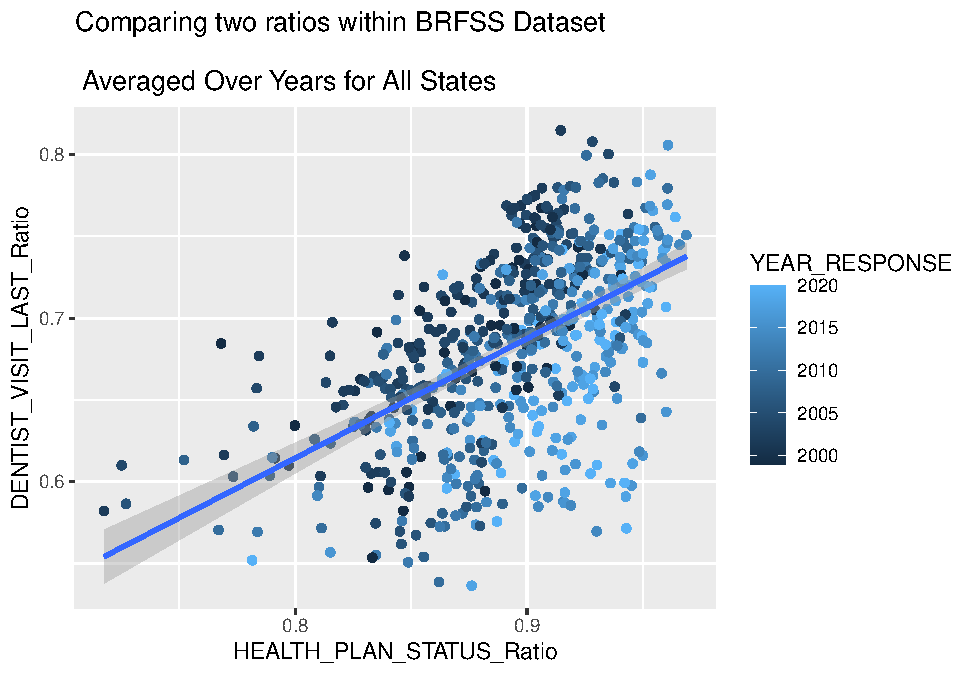
\includegraphics{BRFSS_Graphic_Reproduction_files/figure-latex/unnamed-chunk-6-1.pdf}

There is a list of X and Y variable that possibly be of interest. Note
that you will need to check codebook for their meanings before producing
plots.

\begin{Shaded}
\begin{Highlighting}[]
\NormalTok{XVar\_List }\OtherTok{=} \FunctionTok{c}\NormalTok{(}\StringTok{"ANNUAL\_INCOME\_HSHLD"}\NormalTok{, }\StringTok{"HEALTH\_PLAN\_STATUS"}\NormalTok{, }
              \StringTok{"MED\_COST"}\NormalTok{, }\StringTok{"CHECKUP\_MOST\_RECENT"}\NormalTok{)}
\NormalTok{YVar\_List }\OtherTok{=} \FunctionTok{c}\NormalTok{(}\StringTok{"DENTIST\_VISIT\_LAST"}\NormalTok{, }\StringTok{"NO\_TEETH\_RMVD"}\NormalTok{, }\StringTok{"DENTIS\_CLEAN\_LAST"}\NormalTok{)}
\end{Highlighting}
\end{Shaded}

The following also gives another example plot. The First variable, one
on X-axis, refers to annual household income, specifically the portion
of respondent who have household income of \(\$50,000\) or more. The
Y-axis is Number of Teeth Removed. Var2\_Condition = 8 means that not a
single teeth of the respondent was removed.

\begin{Shaded}
\begin{Highlighting}[]
\FunctionTok{Ratio\_Scatter\_Plotter\_1}\NormalTok{(}\FunctionTok{Data\_Condensor}\NormalTok{(}\AttributeTok{Input\_Data =}\NormalTok{ Data,}
                                        \AttributeTok{Var1 =}\NormalTok{ XVar\_List[}\DecValTok{1}\NormalTok{],}
                                        \AttributeTok{Var2 =}\NormalTok{ YVar\_List[}\DecValTok{2}\NormalTok{],}
                                        \AttributeTok{Var1\_Condition =} \FunctionTok{c}\NormalTok{(}\DecValTok{7}\SpecialCharTok{:}\DecValTok{8}\NormalTok{),}
                                        \AttributeTok{Var1\_Denominator\_Values =} \FunctionTok{c}\NormalTok{(}\DecValTok{1}\SpecialCharTok{:}\DecValTok{8}\NormalTok{),}
                                        \AttributeTok{Var2\_Condition =} \DecValTok{8}\NormalTok{, }
                                        \AttributeTok{Var2\_Denominator\_Values =} \FunctionTok{c}\NormalTok{(}\DecValTok{1}\SpecialCharTok{:}\DecValTok{6}\NormalTok{, }\DecValTok{8}\NormalTok{),}
                                        \AttributeTok{Rename\_Columns =} \ConstantTok{TRUE}\NormalTok{),}
                        \AttributeTok{reverse\_xy\_axis =} \ConstantTok{FALSE}\NormalTok{)}
\end{Highlighting}
\end{Shaded}

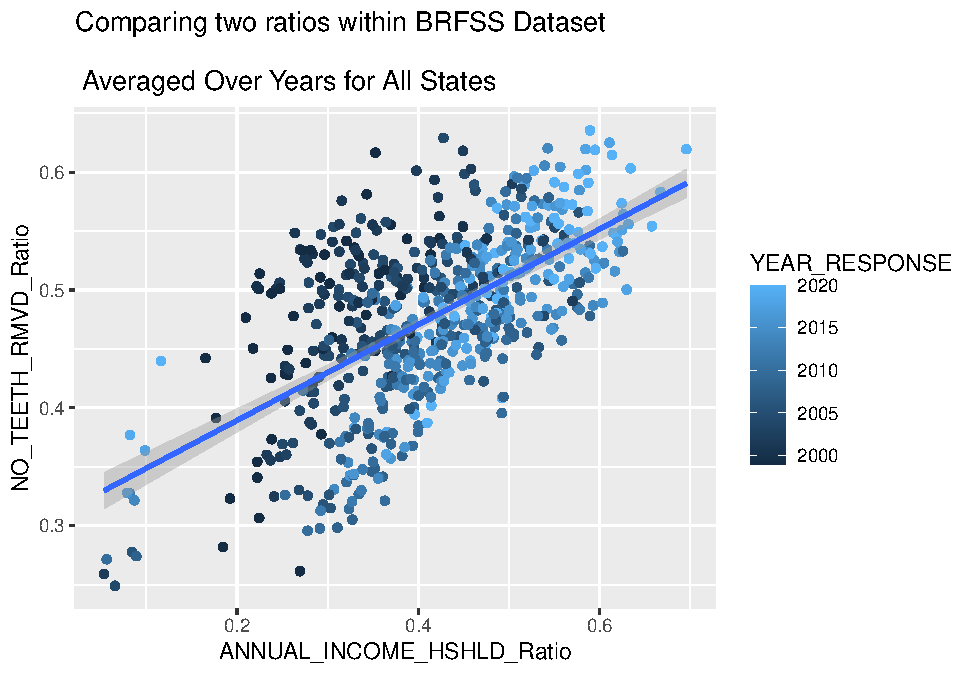
\includegraphics{BRFSS_Graphic_Reproduction_files/figure-latex/unnamed-chunk-8-1.pdf}

It is advised to take notes on the meaning of the ratios upon making
plots. The limited space in X-Y axis means that we cannot put the whole
formula there, and the difference between variables used means
difficulty in providing a coherent formula that works for each
variables.

If you want to make customized entries, As long as you don't have
reverse\_xy\_axis = TRUE the Var1 is always on X-axis and Var2 on
Y-axis. There is a function in ggplot, labs(), that allows customized
label for x and y axis. Add them to the GGPLot section in the function
and it shall show customized labels.

\hypertarget{plotting-averages}{%
\subsection{Plotting Averages}\label{plotting-averages}}

The following function shall plot averages of ratios over state and/or
year, using also processed data. It shall plot a scatterplot but with
averaged ratios on X and Y axis respectively, with a regression line.

Here is the list of variables used:

\begin{quote}
\begin{quote}
Input\_Data: Use a processed dataframe just like the ones above.
\end{quote}
\end{quote}

\begin{quote}
\begin{quote}
return\_average\_of: use average of year, state, or both. Options:
``year'', ``state'', ``both''. Default ``year''
\end{quote}
\end{quote}

\begin{quote}
\begin{quote}
return\_average\_of = ``year'' means that for each year, you get the
averages (of states). = ``state'' means that for each state, return
averages over year. if ``both'' were used, then there would be two
plots.
\end{quote}
\end{quote}

\begin{quote}
\begin{quote}
same Scale: if you used ``both'' in return\_average\_of, then
same\_scale = TRUE means that two resulted plots would be using same x
and y limits, which would be designated immediately following this
variable. If anything else, the scales would not be the same but
automatically decided from each graph. This was used so that it will be
an easier time comparing two plots. Default TRUE
\end{quote}
\end{quote}

\begin{quote}
\begin{quote}
xlim, ylim: both pairs consists a vector of two numbers that limits X
and Y axis. Default is .2 to 1 for both.
\end{quote}
\end{quote}

\begin{quote}
\begin{quote}
Again, the X and Y variables were automatically designated with the
variables ended with ``Ratio''. It can be changed within the function if
you need otherwise.
\end{quote}
\end{quote}

\begin{quote}
\begin{quote}
vertical\_or\_horizontal\_arrange: default ``horizontal. Choose
from''horizontal'' or ``vertical''. tells how the two graphics plotted
would be arranged. Useful only when you put ``both'' in
return\_average\_of.
\end{quote}
\end{quote}

Technical details are included in the comments in the function below.

\begin{Shaded}
\begin{Highlighting}[]
\NormalTok{Ratio\_Scatter\_Plotter\_2 }\OtherTok{=} \ControlFlowTok{function}\NormalTok{(Input\_Data, }
                                   \AttributeTok{return\_average\_of =} \StringTok{"year"}\NormalTok{, }
                                   \AttributeTok{reverse\_xy\_axis =} \ConstantTok{FALSE}\NormalTok{,}
                                   \AttributeTok{same\_scale =} \ConstantTok{TRUE}\NormalTok{, }
                                   \AttributeTok{xlim =} \FunctionTok{c}\NormalTok{(.}\DecValTok{2}\NormalTok{, }\DecValTok{1}\NormalTok{), }\AttributeTok{ylim =} \FunctionTok{c}\NormalTok{(.}\DecValTok{2}\NormalTok{, }\DecValTok{1}\NormalTok{),}
                                   \AttributeTok{vertical\_or\_horizontal\_arrange =} \StringTok{"horizontal"}\NormalTok{)\{}
  
\NormalTok{  List\_of\_Plotting\_Variables }\OtherTok{=} 
    \FunctionTok{colnames}\NormalTok{(Input\_Data)[}\FunctionTok{which}\NormalTok{(}\FunctionTok{grepl}\NormalTok{(}\StringTok{"\_Ratio"}\NormalTok{, }\FunctionTok{colnames}\NormalTok{(Input\_Data)))]}
  \DocumentationTok{\#\# Find the list of variables to be plotted}
  
\NormalTok{  Var1 }\OtherTok{=}\NormalTok{ List\_of\_Plotting\_Variables[}\DecValTok{1}\NormalTok{]}
\NormalTok{  Var2 }\OtherTok{=}\NormalTok{ List\_of\_Plotting\_Variables[}\DecValTok{2}\NormalTok{]}
  
  \ControlFlowTok{if}\NormalTok{(reverse\_xy\_axis)\{}
\NormalTok{    Var1 }\OtherTok{=}\NormalTok{ List\_of\_Plotting\_Variables[}\DecValTok{2}\NormalTok{]}
\NormalTok{    Var2 }\OtherTok{=}\NormalTok{ List\_of\_Plotting\_Variables[}\DecValTok{1}\NormalTok{]}
\NormalTok{  \}}
  \DocumentationTok{\#\#\# Designate the variables for X and Y axis respectively,}
  \DocumentationTok{\#\#\# Which are first and second variables ended in "\_Ratio".}
  \DocumentationTok{\#\#\# Reversed if reverse\_xy\_axis == TRUE.}
  
  \DocumentationTok{\#\#\# Get the year range of data.}
  \DocumentationTok{\#\#\# Since input should be data cleaned by Data\_Condensor,}
  \DocumentationTok{\#\#\# Every year should see data fully available.}
\NormalTok{  Year\_Range }\OtherTok{=} \FunctionTok{unique}\NormalTok{(Input\_Data}\SpecialCharTok{$}\NormalTok{YEAR\_RESPONSE)}
  
  \CommentTok{\# Do averages}
  \ControlFlowTok{if}\NormalTok{(return\_average\_of }\SpecialCharTok{==} \StringTok{"state"}\NormalTok{)\{}
    \CommentTok{\# For state, find average over years.}
    
\NormalTok{    Input\_Data }\OtherTok{=}\NormalTok{  Input\_Data }\SpecialCharTok{\%\textgreater{}\%} \FunctionTok{group\_by}\NormalTok{(STATE\_FIPS\_CODE) }\SpecialCharTok{\%\textgreater{}\%}
      \FunctionTok{summarize}\NormalTok{(}\StringTok{"Var1\_Ave\_Over\_Years"} \OtherTok{=} \FunctionTok{across}\NormalTok{(\{\{ Var1 \}\}, mean), }
                \StringTok{"Var2\_Ave\_Over\_Years"} \OtherTok{=} \FunctionTok{across}\NormalTok{(\{\{ Var2 \}\}, mean)) }\SpecialCharTok{\%\textgreater{}\%}
      \DocumentationTok{\#\#\# Find mean over years, for each state.}
      
      \FunctionTok{mutate}\NormalTok{(}\AttributeTok{Var1\_Ave\_Over\_Years =} \FunctionTok{as.numeric}\NormalTok{(}\FunctionTok{unlist}\NormalTok{(Var1\_Ave\_Over\_Years)), }
             \AttributeTok{Var2\_Ave\_Over\_Years =} \FunctionTok{as.numeric}\NormalTok{(}\FunctionTok{unlist}\NormalTok{(Var2\_Ave\_Over\_Years))) }\SpecialCharTok{\%\textgreater{}\%}
      \DocumentationTok{\#\#\# Use numeric to prevent formatting problems}
      
      \FunctionTok{rename\_at}\NormalTok{(}\FunctionTok{vars}\NormalTok{(}\FunctionTok{c}\NormalTok{(}\StringTok{"Var1\_Ave\_Over\_Years"}\NormalTok{, }\StringTok{"Var2\_Ave\_Over\_Years"}\NormalTok{)),}
                \SpecialCharTok{\textasciitilde{}} \FunctionTok{c}\NormalTok{(}\FunctionTok{paste}\NormalTok{(Var1, }\StringTok{"\_Ave\_Over\_Years"}\NormalTok{, }\AttributeTok{sep =} \StringTok{""}\NormalTok{),}
                    \FunctionTok{paste}\NormalTok{(Var2, }\StringTok{"\_Ave\_Over\_Years"}\NormalTok{, }\AttributeTok{sep =} \StringTok{""}\NormalTok{))) }\SpecialCharTok{\%\textgreater{}\%}
      \DocumentationTok{\#\#\# Rename the variables with character Var1 and Var2 carries}
      \DocumentationTok{\#\#\# Prevent confusion later on}
      
      \FunctionTok{mutate}\NormalTok{(}\AttributeTok{State\_Abb =} \FunctionTok{fips}\NormalTok{(STATE\_FIPS\_CODE, }\AttributeTok{to =}  \StringTok{"Abbreviation"}\NormalTok{)) }\SpecialCharTok{\%\textgreater{}\%}
      \DocumentationTok{\#\#\# Change State FIPS code to abbreviations.}
      
      \FunctionTok{filter}\NormalTok{(STATE\_FIPS\_CODE }\SpecialCharTok{\textless{}=} \DecValTok{56}\NormalTok{) }
    \CommentTok{\# No more Puerto Rico, Virgin Islands, and Guam}
    
    \DocumentationTok{\#\#\# Conduct the plotting.}
    \FunctionTok{ggplot}\NormalTok{(}\AttributeTok{data =}\NormalTok{ Input\_Data,}
           \FunctionTok{aes\_string}\NormalTok{(}\AttributeTok{x =} \FunctionTok{paste}\NormalTok{(Var1, }\StringTok{"\_Ave\_Over\_Years"}\NormalTok{, }\AttributeTok{sep =} \StringTok{""}\NormalTok{), }
               \AttributeTok{y =} \FunctionTok{paste}\NormalTok{(Var2, }\StringTok{"\_Ave\_Over\_Years"}\NormalTok{, }\AttributeTok{sep =} \StringTok{""}\NormalTok{) )) }\SpecialCharTok{+}
      \FunctionTok{geom\_point}\NormalTok{() }\SpecialCharTok{+}
      \FunctionTok{geom\_text}\NormalTok{(}\AttributeTok{label =}\NormalTok{ Input\_Data}\SpecialCharTok{$}\NormalTok{State\_Abb,}
                 \AttributeTok{nudge\_x =} \SpecialCharTok{{-}}\NormalTok{.}\DecValTok{002}\NormalTok{, }\AttributeTok{nudge\_y =}\NormalTok{ .}\DecValTok{001}\NormalTok{) }\SpecialCharTok{+}
      \FunctionTok{ggtitle}\NormalTok{(}\StringTok{"Comparing two ratios within BRFSS Dataset }
\StringTok{              }\SpecialCharTok{\textbackslash{}n}\StringTok{ Averaged Over Years for All States"}\NormalTok{) }\SpecialCharTok{+} 
      \FunctionTok{geom\_smooth}\NormalTok{(}\AttributeTok{method=}\StringTok{\textquotesingle{}lm\textquotesingle{}}\NormalTok{)}
    
\NormalTok{  \}}\ControlFlowTok{else} \ControlFlowTok{if}\NormalTok{(return\_average\_of }\SpecialCharTok{==} \StringTok{"year"}\NormalTok{)\{}
    \CommentTok{\# Average by year, over states.}
\NormalTok{    Input\_Data }\OtherTok{=}\NormalTok{  Input\_Data }\SpecialCharTok{\%\textgreater{}\%} 
      \FunctionTok{filter}\NormalTok{(STATE\_FIPS\_CODE }\SpecialCharTok{\textless{}=} \DecValTok{56}\NormalTok{) }\SpecialCharTok{\%\textgreater{}\%} 
      \CommentTok{\# No more Puerto Rico, Virgin Islands, and Guam}
      
      \FunctionTok{group\_by}\NormalTok{(YEAR\_RESPONSE) }\SpecialCharTok{\%\textgreater{}\%}
      \FunctionTok{summarize}\NormalTok{(}\StringTok{"Var1\_Ave\_Over\_States"} \OtherTok{=} \FunctionTok{across}\NormalTok{(\{\{ Var1 \}\}, mean), }
                \StringTok{"Var2\_Ave\_Over\_States"} \OtherTok{=} \FunctionTok{across}\NormalTok{(\{\{ Var2 \}\}, mean)) }\SpecialCharTok{\%\textgreater{}\%}
      \DocumentationTok{\#\# Make Average over states for each year}
      
      \FunctionTok{mutate}\NormalTok{(}\AttributeTok{Var1\_Ave\_Over\_States =} \FunctionTok{as.numeric}\NormalTok{(}\FunctionTok{unlist}\NormalTok{(Var1\_Ave\_Over\_States)), }
             \AttributeTok{Var2\_Ave\_Over\_States =} \FunctionTok{as.numeric}\NormalTok{(}\FunctionTok{unlist}\NormalTok{(Var2\_Ave\_Over\_States))) }\SpecialCharTok{\%\textgreater{}\%}
      
      \FunctionTok{rename\_at}\NormalTok{(}\FunctionTok{vars}\NormalTok{(}\FunctionTok{c}\NormalTok{(}\StringTok{"Var1\_Ave\_Over\_States"}\NormalTok{, }\StringTok{"Var2\_Ave\_Over\_States"}\NormalTok{)),}
                \SpecialCharTok{\textasciitilde{}} \FunctionTok{c}\NormalTok{(}\FunctionTok{paste}\NormalTok{(Var1, }\StringTok{"\_Ave\_Over\_States"}\NormalTok{, }\AttributeTok{sep =} \StringTok{""}\NormalTok{),}
                    \FunctionTok{paste}\NormalTok{(Var2, }\StringTok{"\_Ave\_Over\_States"}\NormalTok{, }\AttributeTok{sep =} \StringTok{""}\NormalTok{)))}
    
    \DocumentationTok{\#\# Plot with a regression line}
    \FunctionTok{ggplot}\NormalTok{(}\AttributeTok{data =}\NormalTok{ Input\_Data,}
           \FunctionTok{aes\_string}\NormalTok{(}\AttributeTok{x =} \FunctionTok{paste}\NormalTok{(Var1, }\StringTok{"\_Ave\_Over\_States"}\NormalTok{, }\AttributeTok{sep =} \StringTok{""}\NormalTok{), }
                      \AttributeTok{y =} \FunctionTok{paste}\NormalTok{(Var2, }\StringTok{"\_Ave\_Over\_States"}\NormalTok{, }\AttributeTok{sep =} \StringTok{""}\NormalTok{) )) }\SpecialCharTok{+}
      \FunctionTok{geom\_point}\NormalTok{() }\SpecialCharTok{+}
      \FunctionTok{geom\_text}\NormalTok{(}\AttributeTok{label =}\NormalTok{ Input\_Data}\SpecialCharTok{$}\NormalTok{YEAR\_RESPONSE,}
                \AttributeTok{nudge\_x =} \SpecialCharTok{{-}}\NormalTok{.}\DecValTok{002}\NormalTok{, }\AttributeTok{nudge\_y =}\NormalTok{ .}\DecValTok{001}\NormalTok{) }\SpecialCharTok{+}
      \FunctionTok{ggtitle}\NormalTok{(}\StringTok{"Comparing two ratios within BRFSS Dataset }
\StringTok{              }\SpecialCharTok{\textbackslash{}n}\StringTok{ Averaged Over State for All Years"}\NormalTok{) }\SpecialCharTok{+} 
      \FunctionTok{geom\_smooth}\NormalTok{(}\AttributeTok{method=}\StringTok{\textquotesingle{}lm\textquotesingle{}}\NormalTok{)}
\NormalTok{  \}}\ControlFlowTok{else} \ControlFlowTok{if}\NormalTok{(return\_average\_of }\SpecialCharTok{==} \StringTok{"both"}\NormalTok{)\{}
    \CommentTok{\# Plot both stuff above side{-}by{-}side.}
    
\NormalTok{    Part1 }\OtherTok{=}\NormalTok{ Input\_Data}
\NormalTok{    Part2 }\OtherTok{=}\NormalTok{ Input\_Data}
    
    \CommentTok{\# Average over States. Generally the same as above.}
\NormalTok{    Part1 }\OtherTok{=}\NormalTok{ Part1 }\SpecialCharTok{\%\textgreater{}\%} \FunctionTok{group\_by}\NormalTok{(STATE\_FIPS\_CODE) }\SpecialCharTok{\%\textgreater{}\%}
      \FunctionTok{summarize}\NormalTok{(}\StringTok{"Var1\_Ave\_Over\_Years"} \OtherTok{=} \FunctionTok{across}\NormalTok{(\{\{ Var1 \}\}, mean), }
                \StringTok{"Var2\_Ave\_Over\_Years"} \OtherTok{=} \FunctionTok{across}\NormalTok{(\{\{ Var2 \}\}, mean)) }\SpecialCharTok{\%\textgreater{}\%}
      \FunctionTok{mutate}\NormalTok{(}\AttributeTok{Var1\_Ave\_Over\_Years =} \FunctionTok{as.numeric}\NormalTok{(}\FunctionTok{unlist}\NormalTok{(Var1\_Ave\_Over\_Years)), }
             \AttributeTok{Var2\_Ave\_Over\_Years =} \FunctionTok{as.numeric}\NormalTok{(}\FunctionTok{unlist}\NormalTok{(Var2\_Ave\_Over\_Years))) }\SpecialCharTok{\%\textgreater{}\%}
      \FunctionTok{rename\_at}\NormalTok{(}\FunctionTok{vars}\NormalTok{(}\FunctionTok{c}\NormalTok{(}\StringTok{"Var1\_Ave\_Over\_Years"}\NormalTok{, }\StringTok{"Var2\_Ave\_Over\_Years"}\NormalTok{)),}
                \SpecialCharTok{\textasciitilde{}} \FunctionTok{c}\NormalTok{(}\FunctionTok{paste}\NormalTok{(Var1, }\StringTok{"\_Ave\_Over\_Years"}\NormalTok{, }\AttributeTok{sep =} \StringTok{""}\NormalTok{),}
                    \FunctionTok{paste}\NormalTok{(Var2, }\StringTok{"\_Ave\_Over\_Years"}\NormalTok{, }\AttributeTok{sep =} \StringTok{""}\NormalTok{))) }\SpecialCharTok{\%\textgreater{}\%}
      \FunctionTok{mutate}\NormalTok{(}\AttributeTok{State\_Abb =} \FunctionTok{fips}\NormalTok{(STATE\_FIPS\_CODE, }\AttributeTok{to =}  \StringTok{"Abbreviation"}\NormalTok{)) }\SpecialCharTok{\%\textgreater{}\%}
      \FunctionTok{filter}\NormalTok{(STATE\_FIPS\_CODE }\SpecialCharTok{\textless{}=} \DecValTok{56}\NormalTok{) }\CommentTok{\# No more Puerto Rico, Virgin Islands, and Guam}
    
    \CommentTok{\# Average over years. Also generally the same as above}
\NormalTok{    Part2 }\OtherTok{=}\NormalTok{ Part2 }\SpecialCharTok{\%\textgreater{}\%} 
      \FunctionTok{filter}\NormalTok{(STATE\_FIPS\_CODE }\SpecialCharTok{\textless{}=} \DecValTok{56}\NormalTok{) }\SpecialCharTok{\%\textgreater{}\%} 
      \CommentTok{\# No more Puerto Rico, Virgin Islands, and Guam}
      
      \FunctionTok{group\_by}\NormalTok{(YEAR\_RESPONSE) }\SpecialCharTok{\%\textgreater{}\%}
      \FunctionTok{summarize}\NormalTok{(}\StringTok{"Var1\_Ave\_Over\_States"} \OtherTok{=} \FunctionTok{across}\NormalTok{(\{\{ Var1 \}\}, mean), }
                \StringTok{"Var2\_Ave\_Over\_States"} \OtherTok{=} \FunctionTok{across}\NormalTok{(\{\{ Var2 \}\}, mean)) }\SpecialCharTok{\%\textgreater{}\%}
      \FunctionTok{mutate}\NormalTok{(}\AttributeTok{Var1\_Ave\_Over\_States =} \FunctionTok{as.numeric}\NormalTok{(}\FunctionTok{unlist}\NormalTok{(Var1\_Ave\_Over\_States)), }
             \AttributeTok{Var2\_Ave\_Over\_States =} \FunctionTok{as.numeric}\NormalTok{(}\FunctionTok{unlist}\NormalTok{(Var2\_Ave\_Over\_States))) }\SpecialCharTok{\%\textgreater{}\%}
      \FunctionTok{rename\_at}\NormalTok{(}\FunctionTok{vars}\NormalTok{(}\FunctionTok{c}\NormalTok{(}\StringTok{"Var1\_Ave\_Over\_States"}\NormalTok{, }\StringTok{"Var2\_Ave\_Over\_States"}\NormalTok{)), }
                \SpecialCharTok{\textasciitilde{}} \FunctionTok{c}\NormalTok{(}\FunctionTok{paste}\NormalTok{(Var1, }\StringTok{"\_Ave\_Over\_States"}\NormalTok{, }\AttributeTok{sep =} \StringTok{""}\NormalTok{),}
                    \FunctionTok{paste}\NormalTok{(Var2, }\StringTok{"\_Ave\_Over\_States"}\NormalTok{, }\AttributeTok{sep =} \StringTok{""}\NormalTok{)))}
    
\NormalTok{    Part1\_Plot }\OtherTok{=} \FunctionTok{ggplot}\NormalTok{(}\AttributeTok{data =}\NormalTok{ Part1,}
                        \FunctionTok{aes\_string}\NormalTok{(}\AttributeTok{x =} \FunctionTok{paste}\NormalTok{(Var1, }\StringTok{"\_Ave\_Over\_Years"}\NormalTok{, }\AttributeTok{sep =} \StringTok{""}\NormalTok{), }
                            \AttributeTok{y =} \FunctionTok{paste}\NormalTok{(Var2, }\StringTok{"\_Ave\_Over\_Years"}\NormalTok{, }\AttributeTok{sep =} \StringTok{""}\NormalTok{) )) }\SpecialCharTok{+}
      \FunctionTok{geom\_point}\NormalTok{() }\SpecialCharTok{+}
      \FunctionTok{geom\_text}\NormalTok{(}\AttributeTok{label =}\NormalTok{ Part1}\SpecialCharTok{$}\NormalTok{State\_Abb,}
                \AttributeTok{nudge\_x =} \SpecialCharTok{{-}}\NormalTok{.}\DecValTok{002}\NormalTok{, }\AttributeTok{nudge\_y =}\NormalTok{ .}\DecValTok{001}\NormalTok{) }\SpecialCharTok{+}
      \FunctionTok{ggtitle}\NormalTok{(}\StringTok{"Comparing two ratios within BRFSS Dataset }
\StringTok{              }\SpecialCharTok{\textbackslash{}n}\StringTok{ Averaged Over Years for All States"}\NormalTok{) }\SpecialCharTok{+} 
      \FunctionTok{geom\_smooth}\NormalTok{(}\AttributeTok{method=}\StringTok{\textquotesingle{}lm\textquotesingle{}}\NormalTok{)}
    
    
\NormalTok{    Part2\_Plot }\OtherTok{=} \FunctionTok{ggplot}\NormalTok{(}\AttributeTok{data =}\NormalTok{ Part2,}
           \FunctionTok{aes\_string}\NormalTok{(}\AttributeTok{x =} \FunctionTok{paste}\NormalTok{(Var1, }\StringTok{"\_Ave\_Over\_States"}\NormalTok{, }\AttributeTok{sep =} \StringTok{""}\NormalTok{), }
                      \AttributeTok{y =} \FunctionTok{paste}\NormalTok{(Var2, }\StringTok{"\_Ave\_Over\_States"}\NormalTok{, }\AttributeTok{sep =} \StringTok{""}\NormalTok{) )) }\SpecialCharTok{+}
      \FunctionTok{geom\_point}\NormalTok{() }\SpecialCharTok{+}
      \FunctionTok{geom\_text}\NormalTok{(}\AttributeTok{label =}\NormalTok{ Part2}\SpecialCharTok{$}\NormalTok{YEAR\_RESPONSE,}
                \AttributeTok{nudge\_x =} \SpecialCharTok{{-}}\NormalTok{.}\DecValTok{002}\NormalTok{, }\AttributeTok{nudge\_y =}\NormalTok{ .}\DecValTok{001}\NormalTok{) }\SpecialCharTok{+}
      \FunctionTok{ggtitle}\NormalTok{(}\StringTok{"Comparing two ratios within BRFSS Dataset }
\StringTok{              }\SpecialCharTok{\textbackslash{}n}\StringTok{ Averaged Over State for All Years"}\NormalTok{) }\SpecialCharTok{+} 
      \FunctionTok{geom\_smooth}\NormalTok{(}\AttributeTok{method=}\StringTok{\textquotesingle{}lm\textquotesingle{}}\NormalTok{)}
  
    \ControlFlowTok{if}\NormalTok{(same\_scale)\{}
      \DocumentationTok{\#\#\# If using same scales, rearrange the limits to same scales}
\NormalTok{      Part1\_Plot }\OtherTok{=}\NormalTok{ Part1\_Plot }\SpecialCharTok{+} \FunctionTok{xlim}\NormalTok{(xlim[}\DecValTok{1}\NormalTok{], xlim[}\DecValTok{2}\NormalTok{]) }\SpecialCharTok{+} \FunctionTok{ylim}\NormalTok{(ylim[}\DecValTok{1}\NormalTok{], ylim[}\DecValTok{2}\NormalTok{])}
\NormalTok{      Part2\_Plot }\OtherTok{=}\NormalTok{ Part2\_Plot }\SpecialCharTok{+} \FunctionTok{xlim}\NormalTok{(xlim[}\DecValTok{1}\NormalTok{], xlim[}\DecValTok{2}\NormalTok{]) }\SpecialCharTok{+} \FunctionTok{ylim}\NormalTok{(ylim[}\DecValTok{1}\NormalTok{], ylim[}\DecValTok{2}\NormalTok{])}
\NormalTok{    \}}
    \ControlFlowTok{if}\NormalTok{(vertical\_or\_horizontal\_arrange }\SpecialCharTok{==} \StringTok{"horizontal"}\NormalTok{)\{}
      \FunctionTok{grid.arrange}\NormalTok{(Part1\_Plot, Part2\_Plot, }\AttributeTok{ncol =} \DecValTok{2}\NormalTok{)}
      
\NormalTok{    \}}\ControlFlowTok{else} \ControlFlowTok{if}\NormalTok{(vertical\_or\_horizontal\_arrange }\SpecialCharTok{==} \StringTok{"vertical"}\NormalTok{)\{}
      \FunctionTok{grid.arrange}\NormalTok{(Part1\_Plot, Part2\_Plot, }\AttributeTok{nrow =} \DecValTok{2}\NormalTok{)}
\NormalTok{    \}}
    
\NormalTok{  \}}
\NormalTok{\}}
\end{Highlighting}
\end{Shaded}

Here is two examples of the two plots above recreated, but averaged for
both state and year.

For this plot, again X-axis are percentage of people with health
insurance, this time averaged, and Y-axis percentage of people who
visited dentist last year, also averaged. While usually I use horizontal
arrangement, since this is to be used in a PDF document vertical
arrangement should be clearer.

Note that for R Markdown, add fig.height = 16, fig.width=10 in the top
of coding chunk (Like \{r fig.height = 16, fig.width=10\}) when using
vertical plotting of the Ratio\_Scatter\_Plotter\_2 function. Otherwise
the graphic would be compressed too short.

\begin{Shaded}
\begin{Highlighting}[]
\FunctionTok{Ratio\_Scatter\_Plotter\_2}\NormalTok{(}\AttributeTok{Input\_Data =} \FunctionTok{Data\_Condensor}\NormalTok{(}
  \AttributeTok{Input\_Data =}\NormalTok{ Data, }\AttributeTok{Var1 =} \StringTok{"HEALTH\_PLAN\_STATUS"}\NormalTok{, }
  \AttributeTok{Var1\_Condition =} \DecValTok{1}\NormalTok{, }
  \AttributeTok{Var2 =} \StringTok{"DENTIST\_VISIT\_LAST"}\NormalTok{, }
  \AttributeTok{Var2\_Condition =} \DecValTok{1}\NormalTok{, }\AttributeTok{Rename\_Columns =} \ConstantTok{TRUE}\NormalTok{),}
  \AttributeTok{return\_average\_of =} \StringTok{"both"}\NormalTok{,}
  \AttributeTok{reverse\_xy\_axis =} \ConstantTok{FALSE}\NormalTok{,}
  \AttributeTok{same\_scale =} \ConstantTok{TRUE}\NormalTok{,}
  \AttributeTok{xlim =} \FunctionTok{c}\NormalTok{(.}\DecValTok{8}\NormalTok{, .}\DecValTok{95}\NormalTok{),}
  \AttributeTok{ylim =} \FunctionTok{c}\NormalTok{(.}\DecValTok{54}\NormalTok{, .}\DecValTok{82}\NormalTok{),}
  \AttributeTok{vertical\_or\_horizontal\_arrange =} \StringTok{"vertical"}\NormalTok{)}
\end{Highlighting}
\end{Shaded}

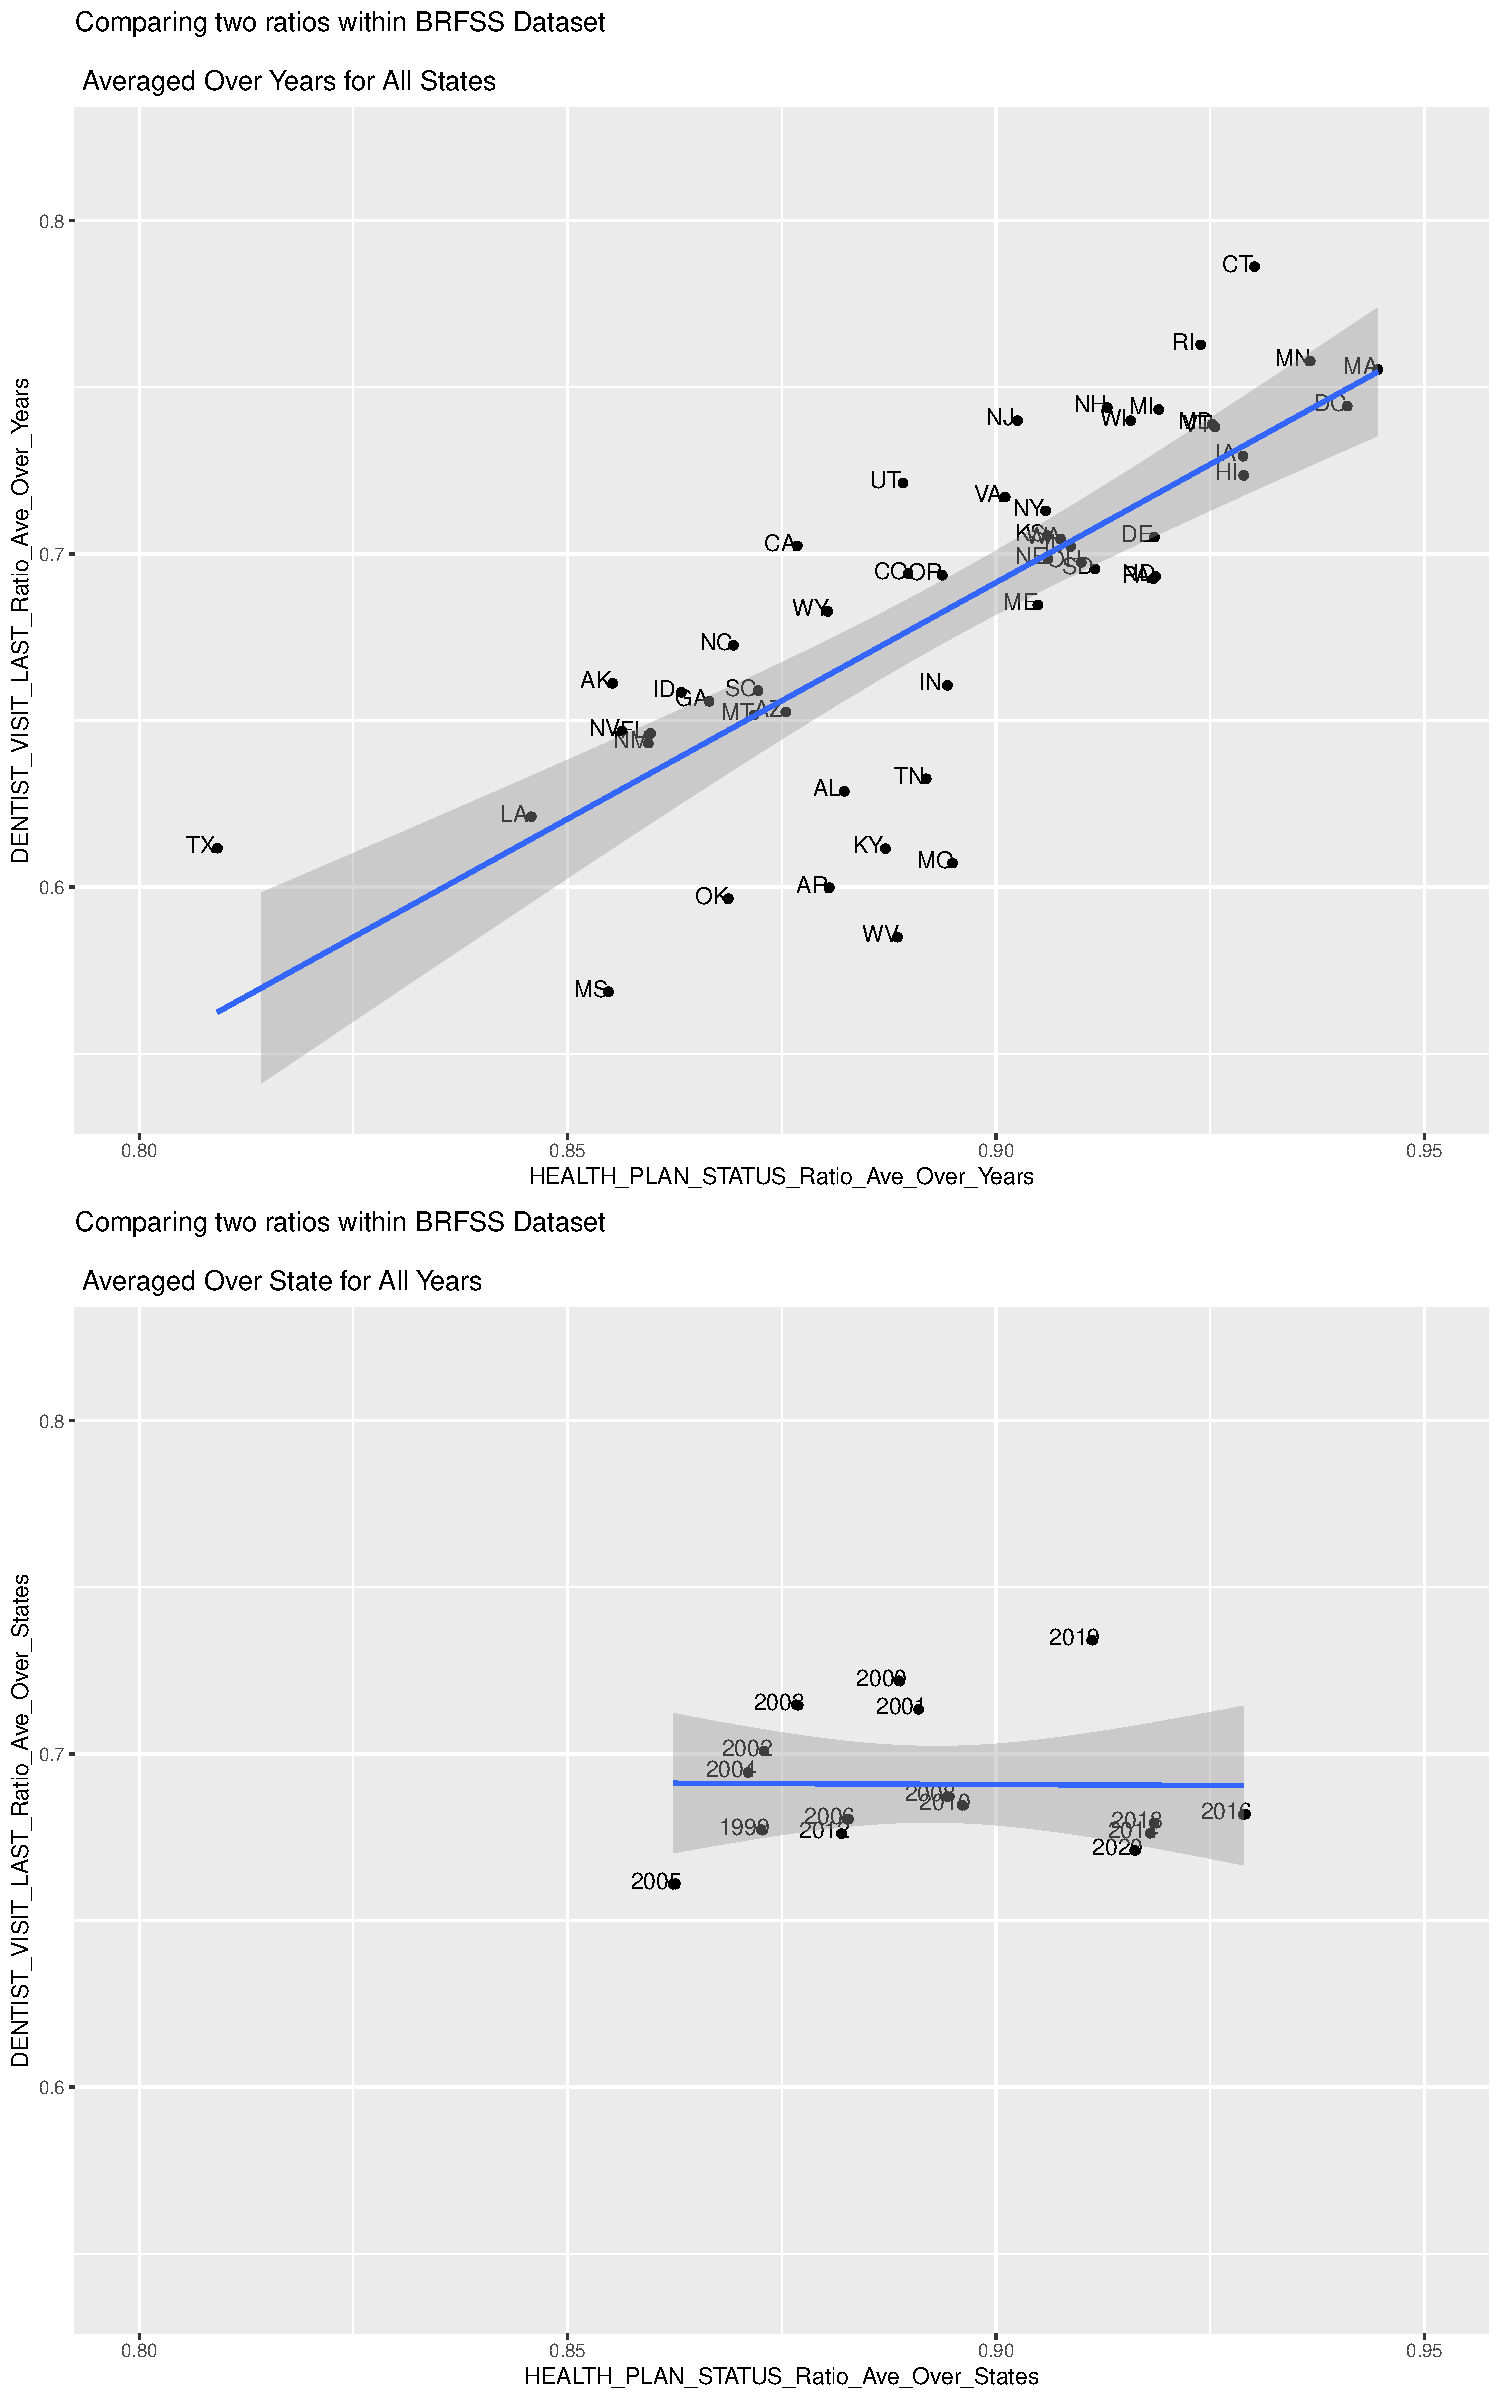
\includegraphics{BRFSS_Graphic_Reproduction_files/figure-latex/unnamed-chunk-10-1.pdf}

For this plot, we have X-axis for people with over \(\$50,000\) annual
income, and Y-axis people who have not a single teeth removed.

\begin{Shaded}
\begin{Highlighting}[]
\FunctionTok{Ratio\_Scatter\_Plotter\_2}\NormalTok{( }\FunctionTok{Data\_Condensor}\NormalTok{(}\AttributeTok{Input\_Data =}\NormalTok{ Data,}
                                        \AttributeTok{Var1 =}\NormalTok{ XVar\_List[}\DecValTok{1}\NormalTok{],}
                                        \AttributeTok{Var2 =}\NormalTok{ YVar\_List[}\DecValTok{2}\NormalTok{],}
                                        \AttributeTok{Var1\_Condition =} \FunctionTok{c}\NormalTok{(}\DecValTok{7}\SpecialCharTok{:}\DecValTok{8}\NormalTok{),}
                                        \AttributeTok{Var1\_Denominator\_Values =} \FunctionTok{c}\NormalTok{(}\DecValTok{1}\SpecialCharTok{:}\DecValTok{8}\NormalTok{),}
                                        \AttributeTok{Var2\_Condition =} \DecValTok{8}\NormalTok{, }
                                        \AttributeTok{Var2\_Denominator\_Values =} \FunctionTok{c}\NormalTok{(}\DecValTok{1}\SpecialCharTok{:}\DecValTok{6}\NormalTok{, }\DecValTok{8}\NormalTok{),}
                                        \AttributeTok{Rename\_Columns =} \ConstantTok{TRUE}\NormalTok{), }
                         \AttributeTok{return\_average\_of =} \StringTok{"both"}\NormalTok{,}
                         \AttributeTok{xlim =} \FunctionTok{c}\NormalTok{(.}\DecValTok{28}\NormalTok{, .}\DecValTok{6}\NormalTok{),}
                         \AttributeTok{ylim =} \FunctionTok{c}\NormalTok{(.}\DecValTok{32}\NormalTok{, .}\DecValTok{58}\NormalTok{),}
                         \AttributeTok{vertical\_or\_horizontal\_arrange =} \StringTok{"vertical"}\NormalTok{)}
\end{Highlighting}
\end{Shaded}

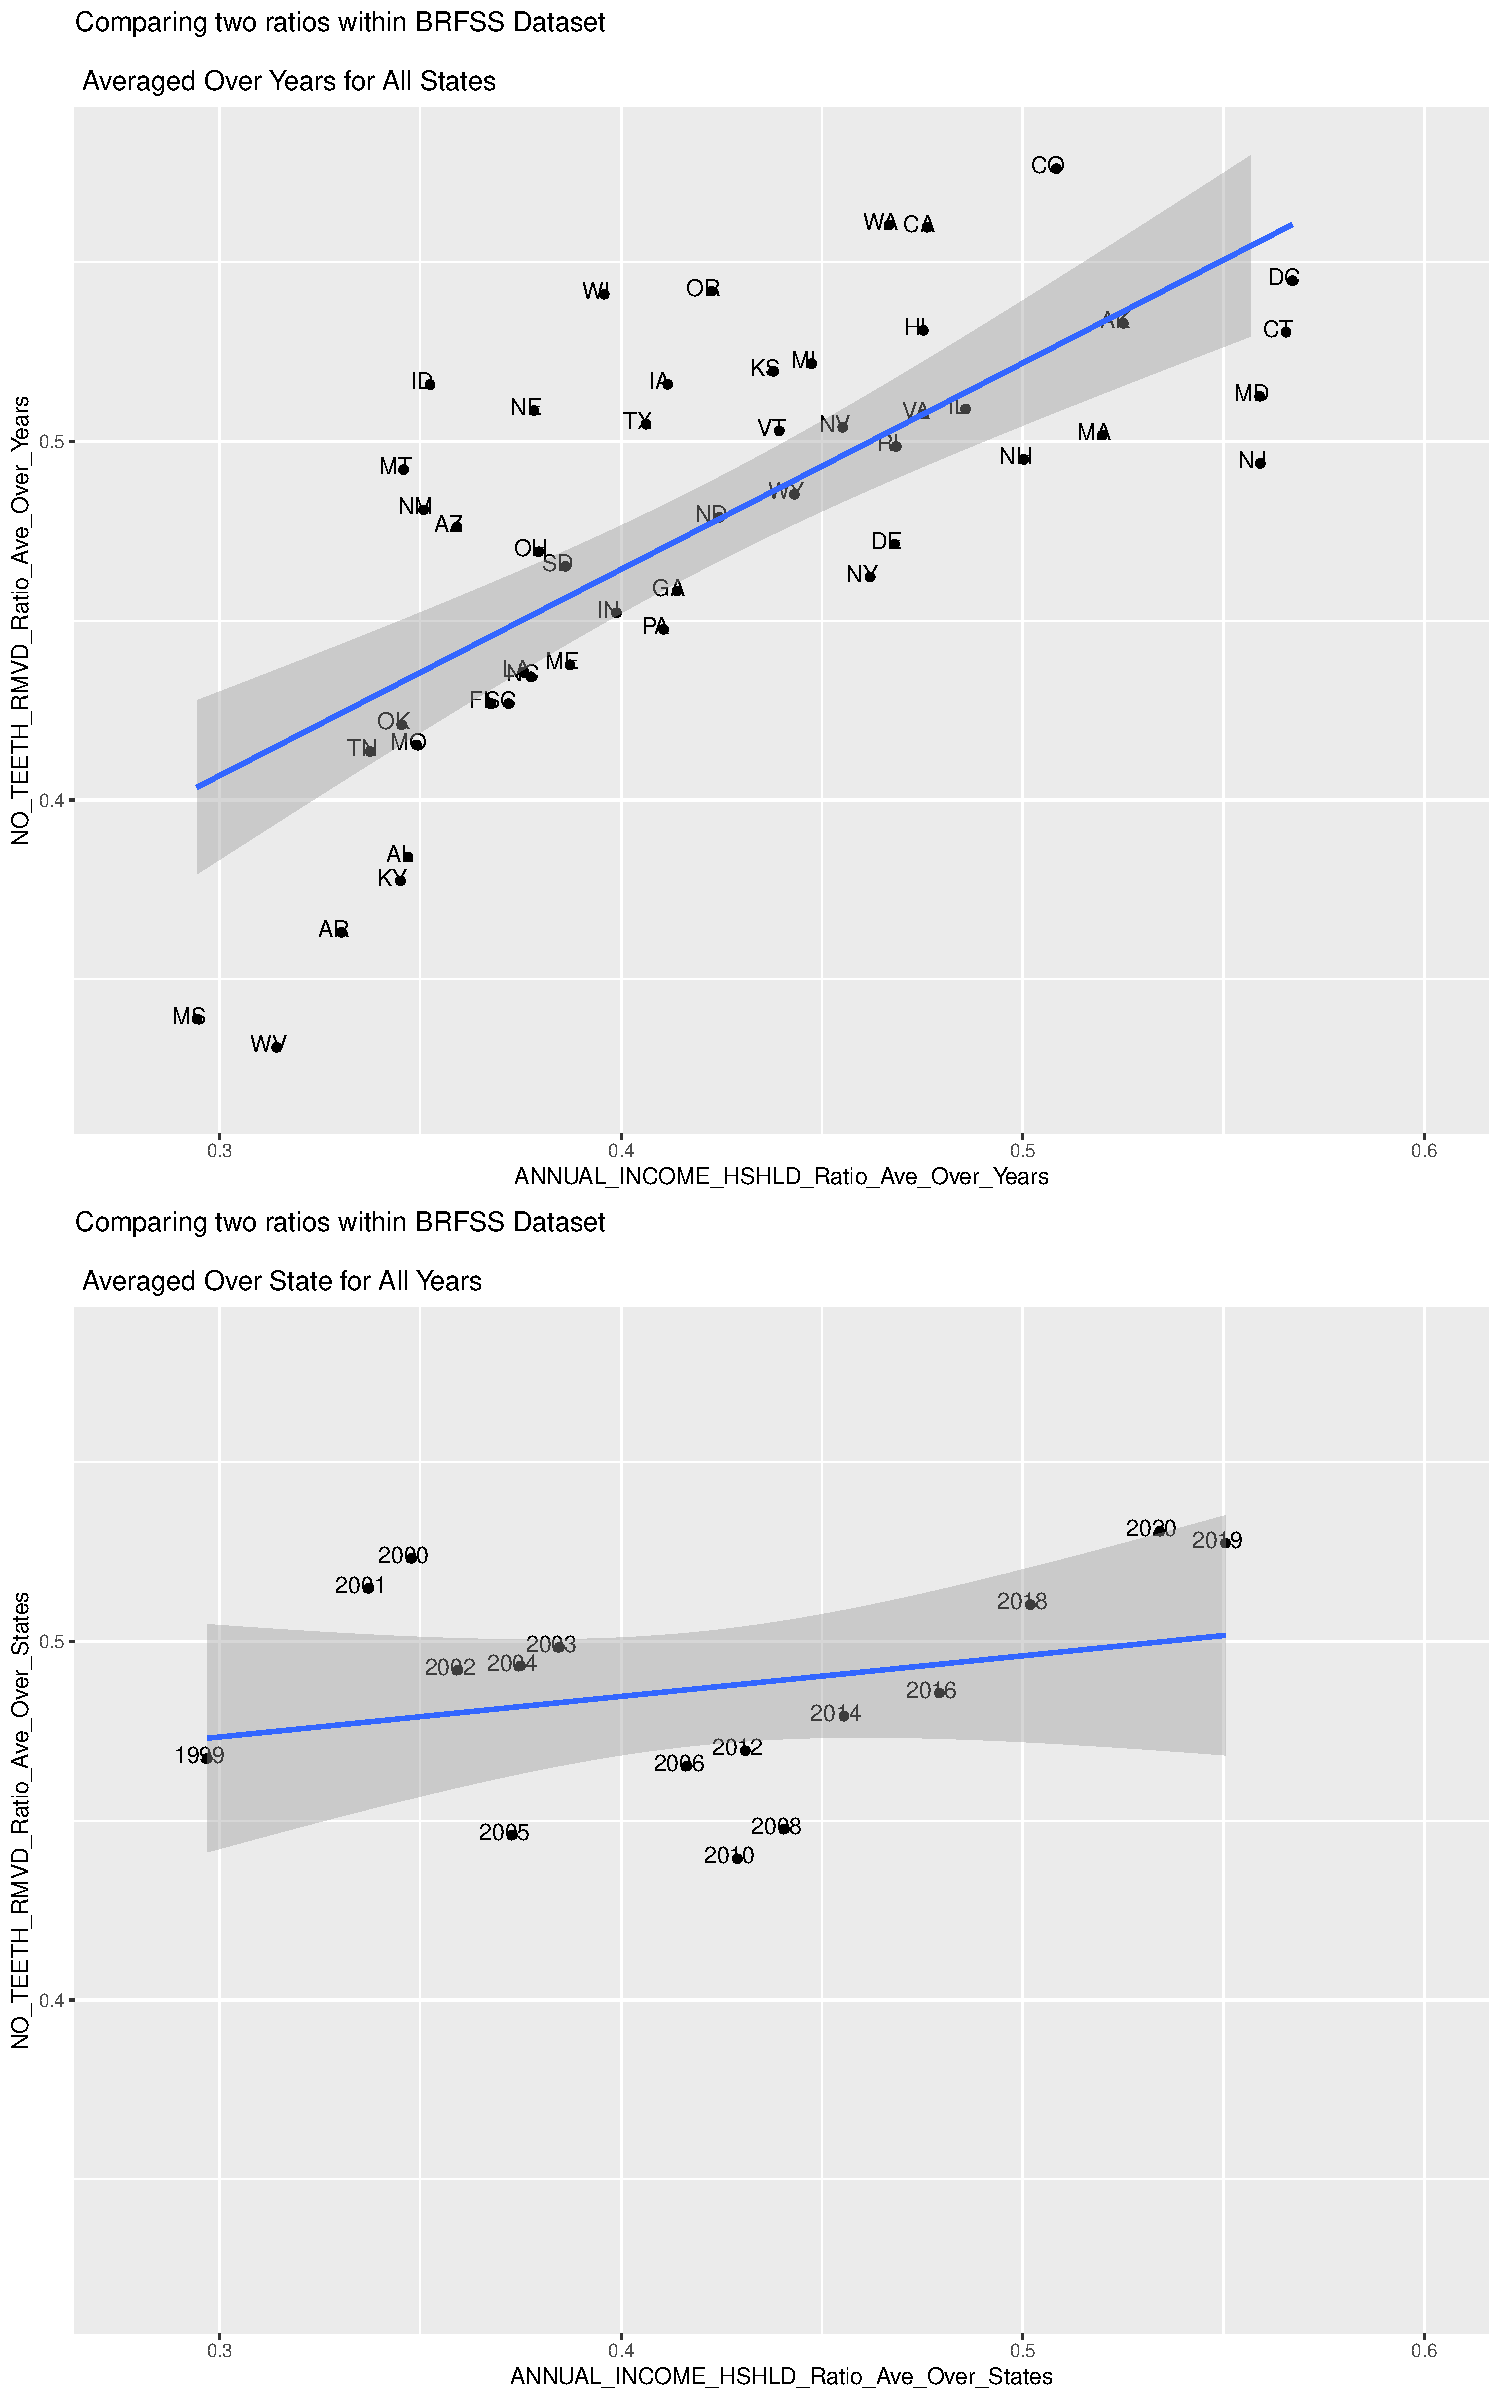
\includegraphics{BRFSS_Graphic_Reproduction_files/figure-latex/unnamed-chunk-11-1.pdf}

Feel free to use Codebook and the function to create even more plots to
be used!

\end{document}
